\section{Theoretischer Hintergrund}
\subsection{Oszilloskop}
Bei einem Oszilloskop handelt es sich um ein Messgerät das Spannungen in Funktion der Zeit erfassen und grafisch darstellen kann. Man unterscheidet zwischen \textbf{Analoges} und \textbf{Digitales Oszilloskop}. Meistens sind zwei Messkanäle (Channel, Ch) vorhanden. Achtung: beide Kanäle messen auf einen gemeinsamen
Bezugspunkt!. 
\subsubsection{Analoges Oszilloskop}
Auch \textbf{Kathodenstrahl Oszilloskop} oder abgekürzt \textbf{KO} genannt. Die zu messende Spannung wird verstärkt und steuert direkt den Elektronenstrahl der Kathodenstrahlröhre (cathode ray tube, CRT) an. Systembedingt kann das Gerät i.d.R. nur periodische und repetierende Signale erfassen. Eine Speichermöglichkeit der erfassten Messspannung besteht - ausser bei speziellen (teuren) Ko's - nicht.
\subsubsection{Digitales Oszilloskop}
Auch \textbf{Digitales Speicher Oszilloskop} oder abgekürzt \textbf{DSO} genannt. Das Messsignal wird hier zuerst mit einem Analog-Digital-Converter (ADC) digitalisiert und in einem Speicher abgelegt. Anschliessend werden die Daten vom messgerätinternen Rechner verarbeitet und auf der Anzeigeeinheit, meist einem Liquide Crystal Display (LCD), dargestellt. Da die Messwerte digitalisiert und gespeichert werden, eignet sich das DSO auch für nicht repetierende Signale (single shot Messungen). Wenn bei der Digitalisierung die Abtastfrequenz (sampling rate) nicht mindestens der doppelten Messfrequenz entspricht, kommt es zu Aliasingeffekten. Typische Abtastfrequenzen liegen beim 10- bis 20-fachem der Messfrequenz.
\\\\
Im Labor arbeiten wir mit dem Tektronix Digital Scope TDS3014B. Tektronix ist einer der führenden Hersteller von Oszilloskopen.
\\\\
In einer Schaltung ist es meist am besten, die Signale mit einem Tastkopf (Sonde) an den DSO-Input anzuschliessen. Tastköpfe haben in der Regel einen 10-fach (selten 100-fach) Spannungsteiler eingebaut. Dafür steigt die Eingangsimpedanz um den Faktor 10 (bzw. 100) an. Ziehen Sie den vorderen Teil einer Sonde nie ab, da ihre Spitze (Steckkontakt) so ungeschützt ist und beschädigt werden kann.
\subsection{Funktionsgenerator}
Mit dem Funktionsgenerator (FG) lassen sich spezielle elektrische Spannungsverläufe erzeugen. In der Regel sind dies:
\begin{enumerate}[$a)$]
\item Sinus
\item Rechteck
\item Dreieck
\item Sägezahn
\item Puls
\end{enumerate}
Die Parameter: Amplitude, Frequenz, Offset und Tastverhältnis lassen sich gezielt einstellen. Unter \textbf{Offset} versteht man die Addition einer Gleichspannung zum obigen Signalverlauf. Das Tastverhältnis oder \textbf{Duty Cycle} $g$ kommt nur beim Rechtecktsignal vor. Es entspricht dem Verhältnis der Impulsdauer $t_i$ zu Periodendauer $T$ und wird meistens in \% angegeben
\begin{equation}
\boxed{g=\dfrac{t_i}{T}}
\end{equation}
\begin{center}
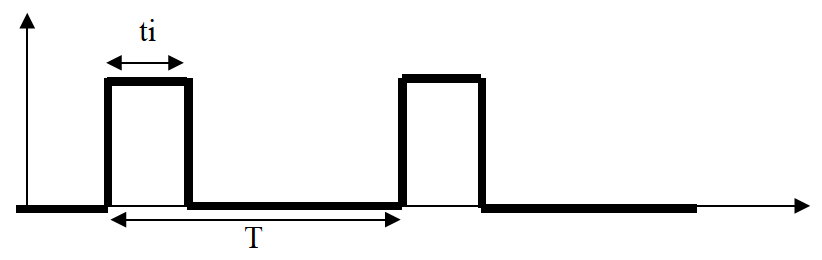
\includegraphics[scale=0.5]{../img/IV/IVd}
\end{center}
Zudem kann der FG vom Labor auch modulierte Signale und beliebige Signalformen ausgeben. Im Labor wird mit dem FG vomTyp Tektronix AFG1062 gearbeitet.
\subsection{RC-Glied}
\subsubsection{Der Kondensator $C$}
Ein Kondensator besteht aus zwei elektrisch leitenden Platten, die durch eine Isolation (Dielektrikum) getrennt sind. Beim Anschlussan eine Gleichspannung $U_0$ entzieht diese der einen Platte Elektronen und drückt sie auf die andere Platte. Der Kondensator wird dadurch geladen. Während der Ladezeit fliesst in den Zuleitungen ein Strom $i_C\left(t\right)$, obwohl zwischen den Platten kein Strom fliesst. Wenn $u_C\left(t\right)=U_0$ geworden ist, ist die Ladung beendet, und somit wird $i_C\left(t\right)=0$. Die Energie bleibt im Kondensator erhalten (gespeichert), auch wenn dieser von der Speisequelle abgetrennt wird. Das Fassungsvermögen des Kondensators heisst \textbf{Kapazität} und hat die Einheit Farad [F]=[AsV$^{-1}$].  
\\\\
Ein Kondensator $C$ besitzt per Definition die Kapazität $1\text{F}$, wenn er bei einer gespeicherten Ladung $Q$ von einem Coulomb ($1\text{C}=6.24\cdot 10^{18}\text{ Elektronen}$) auf $1\text{V}$ geladen wird. Elektrolytkondensatoren sind gepolt und dürfen nicht verkehrt angeschlossen werden. Allgemein gilt
\begin{equation}
\boxed{i_C\left(t\right)=C\cdot \dfrac{\text{d}}{\text{d}t}u_C\left(t\right)}\quad \boxed{u_C\left(t\right)=\dfrac{1}{C}\displaystyle \int i_C\left(t\right)\,\text{d}t}
\end{equation}
\subsubsection{Vereinfachung}
Wenn im Zeitintervall $\triangle t$ der Strom $i_C\left(t\right)$ als konstant zu $I_C$ angenommen wird (Gleichstrombetrachtung), darf man schreiben
\begin{equation}
\boxed{C=\dfrac{\triangle Q}{\triangle U_C}}\quad \boxed{I_C=C\cdot \dfrac{\triangle U_C}{\triangle t}}
\end{equation}
\subsubsection{Überlegung}
Wie verläuft die Spannung $U_C$ über einem Kondensator $C$, wenn er mit einem konstanten Strom $I_C$ geladen wird? Annahme: zum Zeitpunkt $t=0$ sei der Kondensator entladen: $U_C=0\text{V}$.
\begin{center}
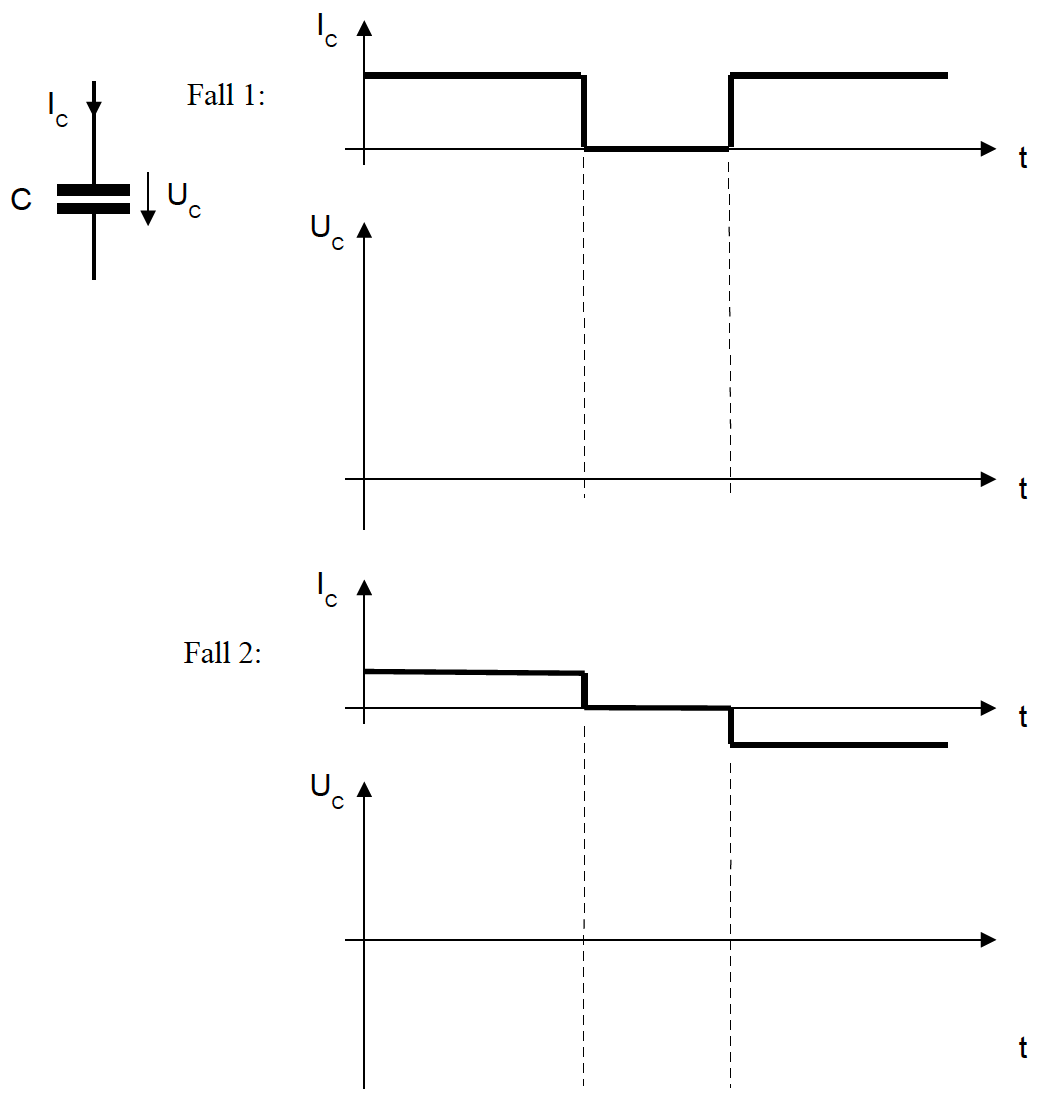
\includegraphics[scale=0.5]{../img/IV/IVe}
\end{center}
\subsubsection{Impulsverhalten von RC-Gliedern}
Wie sieht der Spannungsverlauf über dem Kondensator $u_C\left(t\right)$ aus, wenn er über einen Schalter und einen Widerstand $R$ an eine Gleichspannung $U_0$ angeschlossen wird?
\begin{center}
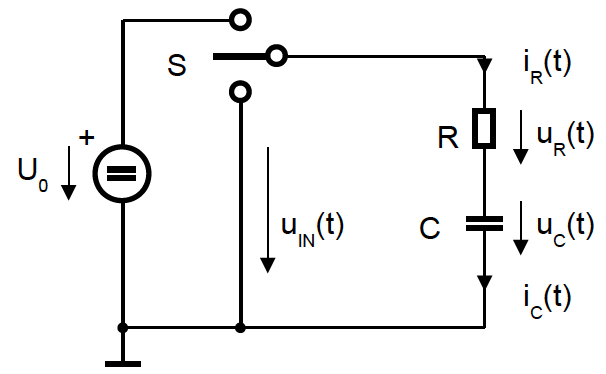
\includegraphics[scale=0.5]{../img/IV/IVf}
\end{center}
Bsp: Gegeben $U_0=10\text{V}$, $R=1\text{k}\Omega$, $C=0.1\mu\text{F}$, $U_C\left(t\right)=0\text{V}$. Gesucht: $u_C\left(t\right)$ und $i_C\left(t\right)$
\\\\
Mit der Beziehung 
\begin{equation}
\boxed{C\cdot \triangle u_C\left(t\right)=i_C\left(t\right)\cdot \triangle t=\triangle Q\left(t\right)}
\end{equation}
kann man nun in Intervallen $\triangle t$ zu diskreten Zeitpunkten $t_n$ die jeweiligen Werte numerische berechnen. Annahme: der Strom $i_C\left(t\right)$ bleibt in einem Zeitintervall $\triangle t$ konstant.
\begin{equation*} 
\begin{array}{lll} 
u_R\left(t_n\right)&=&U_0-u_C\left(t_n\right)\\
i_C\left(t_n\right)&=&i_R\left(t_n\right)=\dfrac{u_R\left(t\right)}{R}\\
\triangle u_C\left(t_n\rightarrow t_{n+1}\right)&=&i_C\left(t_n\right)\cdot \dfrac{\triangle t}{C}\\
u_C\left(t_{n+1}\right)&=&u_C\left(t_n\right)+\triangle u_C\left(t_n\rightarrow t_{n+1}\right)
\end{array} 
\end{equation*} 
Folgende Werte sind für den \textbf{Ladevorgang} für eine Zeitdauer von $100\mu\text{s}$
\begin{center} 
\begin{tabular}{|c|c|c|c|c|}\hline
$t_n/\mu\text{s}$&$\triangle u_C\left(t_n\rightarrow t_{n+1}\right)$&$u_C\left(t\right)$&$u_R\left(t_n \right)$&$i_C\left(t_n \right)$\\\hline
0&&&&\\
20&&&&\\
40&&&&\\
60&&&&\\
80&&&&\\
100&&&&\\\hline
\end{tabular}
\end{center}
Folgende Werte sind für den \textbf{Entladevorgang} für eine Zeitdauer von $100\mu\text{s}$
\begin{center} 
\begin{tabular}{|c|c|c|c|c|}\hline
$t_n/\mu\text{s}$&$\triangle u_C\left(t_n\rightarrow t_{n+1}\right)$&$u_C\left(t\right)$&$u_R\left(t_n \right)$&$i_C\left(t_n \right)$\\\hline
0&&&&\\
20&&&&\\
40&&&&\\
60&&&&\\
80&&&&\\
100&&&&\\\hline
\end{tabular}
\end{center}
\begin{center}
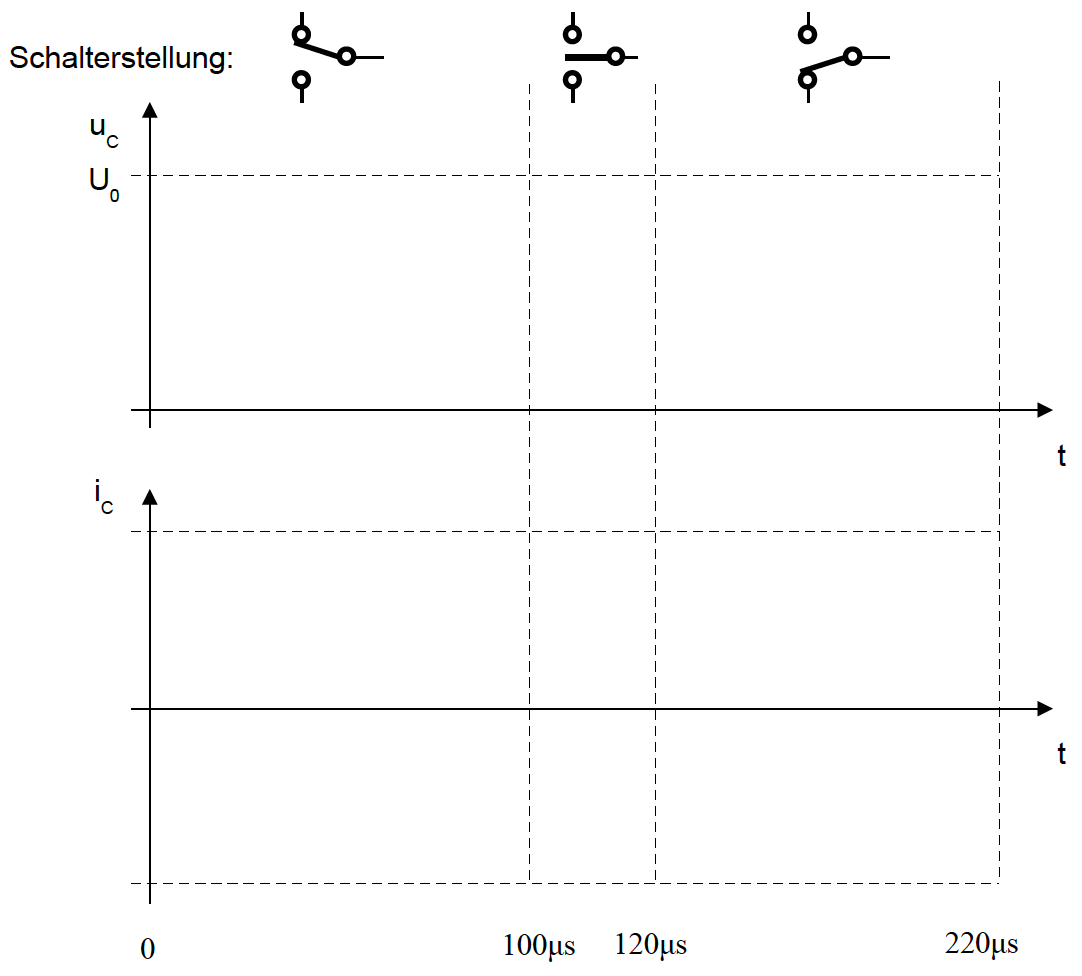
\includegraphics[scale=0.45]{../img/IV/IVg}
\end{center}
Der genaue Verlauf der Spannung resp. des Stromes in Kondensator lässt sich beim \textbf{Aufladen} folgendermassen berechnen.
\begin{equation}
\boxed{u_C\left(t\right)=U_0\cdot \left(1-e^{-\dfrac{t}{\tau}}\right)}
\end{equation}
$\tau$ ist die \textbf{Zeitkonstante} und berechnet sich zu
\begin{equation}
\boxed{\tau=R\cdot C}
\end{equation}
Nach einer Zeitkonstanten $t=1\tau$ hat sich der Kondensator auf $63\%$ von $U_0$ aufgeladen.
\begin{equation}
\boxed{i_C\left(t\right)=I_0\cdot e^{-\dfrac{t}{\tau}}}
\end{equation}
Der \textbf{Anfangsstrom} $I_0$ berechnet sich zu
\begin{equation}
\boxed{I_0=\dfrac{U_0}{R}}
\end{equation}
Nach $t=1\tau$ ist der Strom auf $37\%$ abgesunken. Nach $t=5\tau$ ist der Ladevorgang praktisch abgeschlossen $(u_C\approx 100\%, i_C\approx 0)$
\\\\
Bei der \textbf{Entladung} gelten die folgenden Formel
\begin{equation}
\boxed{u_C\left(t\right)=U_0\cdot e^{-\dfrac{t}{\tau}}}\quad \boxed{i_C\left(t\right)=-I_0\cdot e^{-\dfrac{t}{\tau}}}
\end{equation}
Die Spannung $u_R\left(t\right)$ über dem Widerstand $R$ verläuft in beiden Fällen proportional zum Strom $i_C\left(t\right)$
\begin{equation}
\boxed{u_R\left(t\right)=i_C\left(t\right)\cdot R}
\end{equation}
\subsection{Zusammenfassung: Impulsverhalten von RC-Gliedern}
\begin{center}
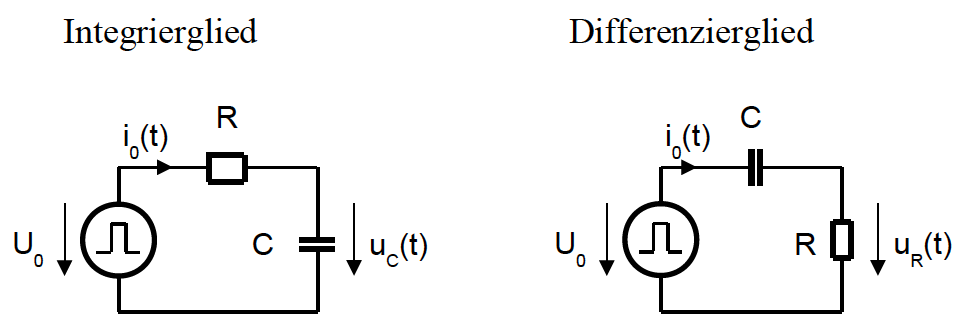
\includegraphics[scale=0.5]{../img/IV/IVh}
\end{center}
\begin{center}
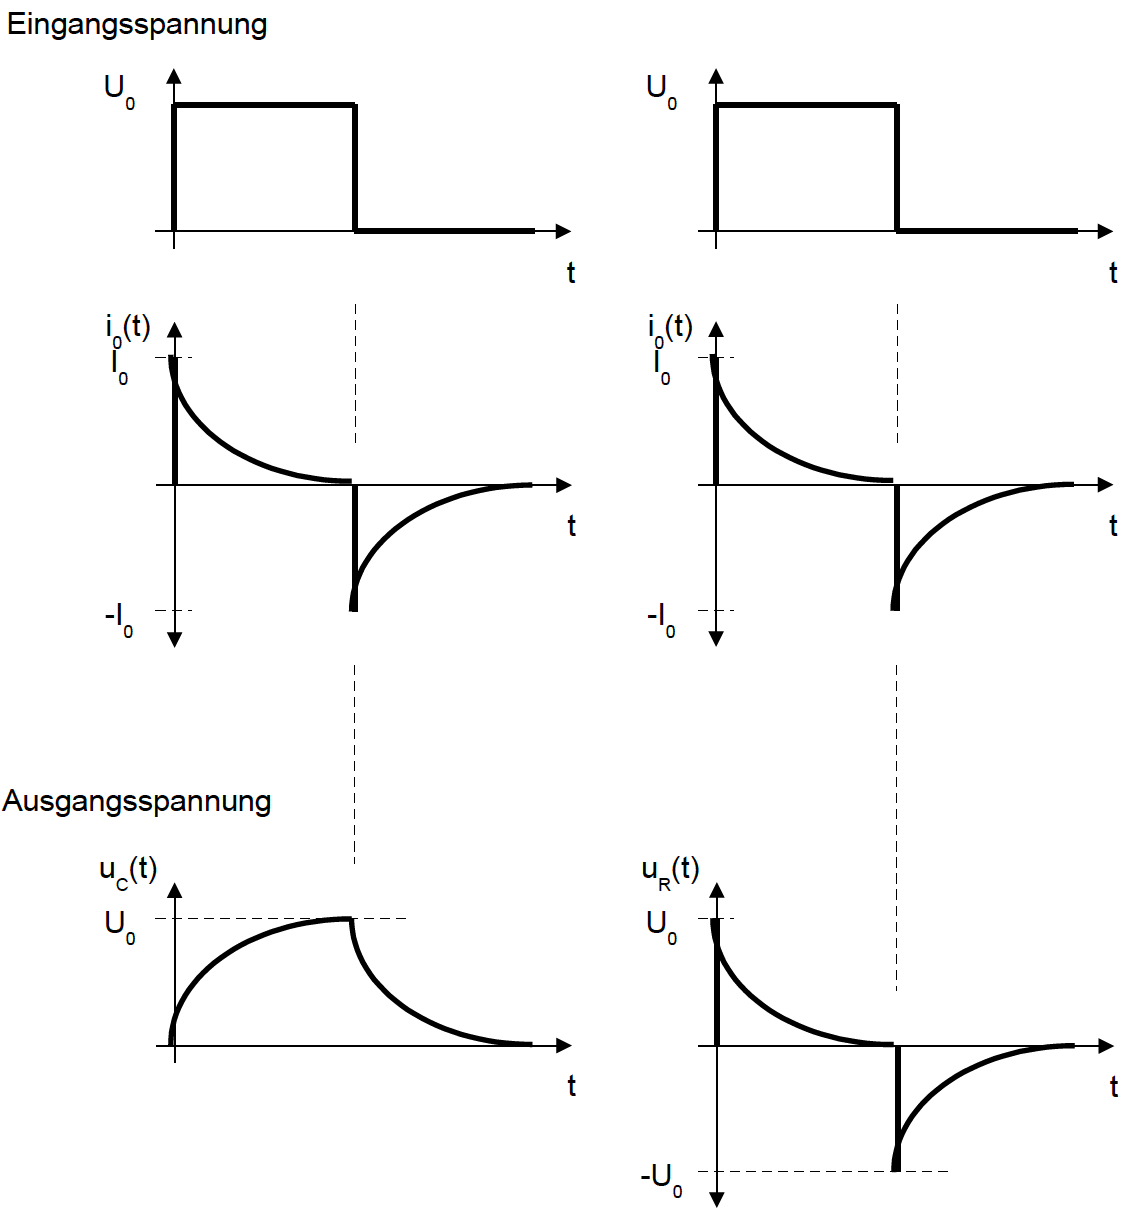
\includegraphics[scale=0.45]{../img/IV/IVj}
\end{center}
\subsection{Begriffe des KO}
\textbf{Division:} Teilung oder Abschnitt des Bildschirmgitters; früher oft als Zentimeter („10mV/cm“) bezeichnet.
\\\\
\textbf{DC:} engl. Direct Current = Gleichspannung/Gleichstrom.
\\\\
\textbf{AC:} engl. Alternating Current = Wechselspannung / Wechselstrom.
\\\\
\textbf{GND:} engl. Ground = Massepotential, Nullpotential.
\\\\
\textbf{HF:} engl. High Frequency = Hochfrequenz.
\\\\
\textbf{Line:} engl. Begriff für Stromnetz-Bezug, aktuelle Netzfrequenz (50 Hz).
\\\\
\textbf{Video, TV:} Aktivieren eines Filters im Triggerverstärker, das aus einem Videosignal das Zeilenwechselsignal als Trigger herausfiltert.
\\\\
\textbf{Frame:} Aktivieren eines Filters im Triggerverstärker, das aus einem Videosignal das Bildwechselsignal als Trigger. herausfiltert
\\\\
\textbf{Slope:} eng. für Flanke, der steigende oder fallende Abschnitt einer periodischen Funktion, der das Triggersignal auslöst.
\\\\
\textbf{Delay:} engl. für Verzögerung, die zeitliche Verzögerung zwischen Triggerzeitpunkt und Beginn der Bilddarstellung, die ermüglicht, das Ereignis zu zeigen, das den Trigger ausgelüst hat.
\\\\
\textbf{Trigger:} Auslüsesignal, das das Zeichnen des Schirmbildes veranlasst.
\subsection{Kopplungsarten}
Stellt man den Eingangswahlschalter auf \textbf{DC}, so besteht eine \textbf{Gleichspannungskopplung} zum Verstärker des Oszilloskops. Damit wird sowohl der Gleichspannungsanteil wie auch der Wechselspannungsanteil des Signals auf dem Schirm korrekt angezeigt. 
\\\\
Will man hingegen nur den \textbf{veränderlichen Anteil}, z.B. die Rippelspannung einer Gleichspannung, darstellen und den Gleichanteil unterdrücken, kann mit der Schalterstellung \textbf{AC} eine Wechselspannungskopplung des Eingangs bewirkt werden.
\\\\
Die neue \textbf{Null-Linie} des Schirmbildes entsteht beim (linearen) Mittelwert der Kurvenform der Signalspannung, ein eventuell vorhandener Gleichspannungsanteil wird unterdrückt. 
\\\\
Bei sehr langsamen Vorgängen können in der Stellung AC Verzerrungen der Kurvenform auftreten.
\begin{center}
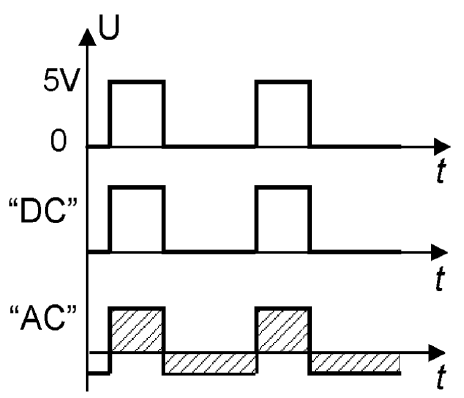
\includegraphics[scale=0.75]{../img/IV/IVa}
\end{center}
\subsection{Tastköpfe und Messonden}
\begin{center}
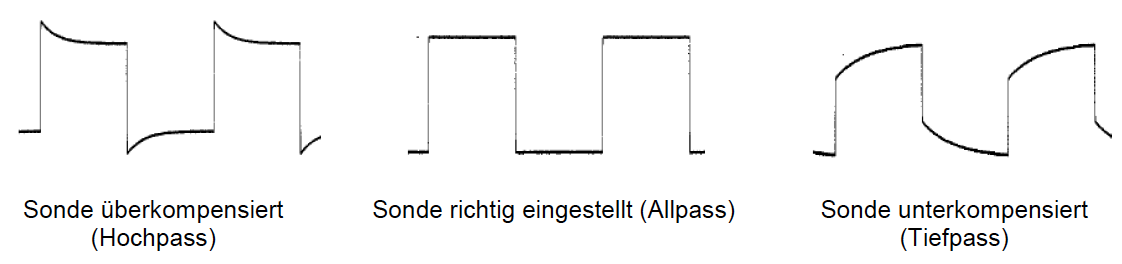
\includegraphics[scale=0.4]{../img/IV/IVb}
\end{center}
\begin{center}
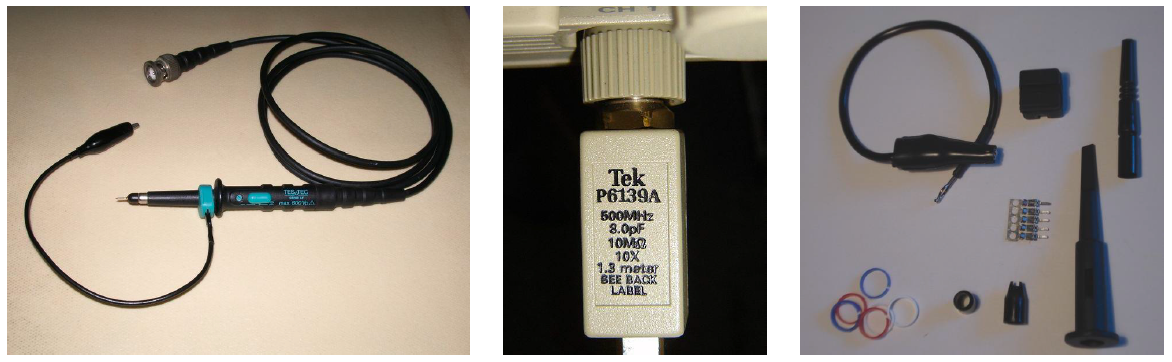
\includegraphics[scale=0.4]{../img/IV/IVc}
\end{center}
\section{Versuchsanleitung}
\subsection{Theoretische Aufgaben}
\begin{enumerate}[$a)$]
\item Sie möchten von einer \textbf{DC Spannung} von $15\text{V}$ die \textbf{Rippelspannung} messen.
\begin{enumerate}[$\bullet$]
\item In welchem Bereich ist so eine Rippelspannung zu erwarten?
\item Mit welcher Kopplungsart messen Sie die Rippelspannung?
\end{enumerate}
\item Was können Sie mit AC-Kopplung nicht messen?
\item Was kann derNachteil einer AC-Kopplung sein?
\item Wieso verwendet man Messonden?
\item Was ist der Nachteil einer Messonde?
\end{enumerate}
\subsection{Versuchsinhalt}
Die meisten elektrischen Vorgänge verlaufen in Funktion der Zeit variabel und können damit nicht mit einem digitalen Multimeter (DMM) erfasst werden.
\\\\
Im ersten Teil des Versuchs lernt man den Umgang mit dem \textbf{Oszilloskop} und dem \textbf{Funktionsgenerator} kennen. Als Anwendung will man im zweiten Teil das \textbf{Impulsverhalten
eines RC-Gliedes} mit diesen beiden Geräten ausmessen.
\subsection{Ziel des Versuchs}
Ziele des Versuchs sind
\begin{enumerate}[$a)$]
\item Funktionsweiseund Bedienung des Oszilloskops verstehen.
\item Richtige Anwendung des Oszilloskops für alle späteren Versuche kennen lernen.
\item Generierung elementarer Signale mit dem Funktionsgenerator.
\item Ausmessen eines RC-GliedesimZeitbereich als Integrierer und Differenzierer.
\end{enumerate}
\subsection{Inbetriebnahme von FG und DSO}
\subsubsection{Vorbereitungen}
\begin{enumerate}[$a)$]
\item Verbinden Sie den Ausgang des Funktionsgenerators (FG) HP 33120A mit dem Vertikaleingang CH1 des Oszilloskops (DSO) TDS3014B mit einer 1:10-Sonde.
\item Stellen Sie am FG die Signalform auf Sinus, die Amplitude auf 5.0Vpp, die Frequenz auf 1kHz und drücken Sie auf dem DSO die Taste ``AUTOSET''. Jetzt sollten Sie ein stehendes Bild auf der DSO-Anzeige haben.
\item Verstellen Sie auf dem FG die Kurvenform (Sinus, Dreieck, Rechteck) und kontrollieren Sie sie auf dem DSO.
\end{enumerate}
\subsubsection{Aufgabe 1}
\begin{enumerate}[$\bullet$]
\item Stellen Sie am FG eine Sinusspannung von 1.0Vpp (Spitzen-Spitzen Wert) und einer Frequenz von 10kHz ein. 
\item Der Offset am FG muss 0 sein, es darf kein "Offset" im Display des FG erscheinen.
\item Messen Sie die Werte mit dem DSO. Machen Sie die Einstellungen mit den beiden „SCALE“-Drehknöpfen, nicht mit der "AUTOSET"-Taste. 
\item Verwenden Sie auch die "CURSOR"-Möglichkeiten des DSO. 
\item Frage: Wie gross sind die Abweichungen der gemessenen Werte von den Einstellungen am FG? (Angaben in \%) 
\item Stellen Sie sicher, dass die Anschlüsse des FG und des DSO auf High-Z resp. $1\text{M}\Omega$ eingestellt sind.
\end{enumerate}
\subsection{RC-Glieder}
\section{Diskussion}